\documentclass[11pt]{article}

    \usepackage[breakable]{tcolorbox}
    \usepackage{parskip} % Stop auto-indenting (to mimic markdown behaviour)
    

    % Basic figure setup, for now with no caption control since it's done
    % automatically by Pandoc (which extracts ![](path) syntax from Markdown).
    \usepackage{graphicx}
    % Keep aspect ratio if custom image width or height is specified
    \setkeys{Gin}{keepaspectratio}
    % Maintain compatibility with old templates. Remove in nbconvert 6.0
    \let\Oldincludegraphics\includegraphics
    % Ensure that by default, figures have no caption (until we provide a
    % proper Figure object with a Caption API and a way to capture that
    % in the conversion process - todo).
    \usepackage{caption}
    \DeclareCaptionFormat{nocaption}{}
    \captionsetup{format=nocaption,aboveskip=0pt,belowskip=0pt}

    \usepackage{float}
    \floatplacement{figure}{H} % forces figures to be placed at the correct location
    \usepackage{xcolor} % Allow colors to be defined
    \usepackage{enumerate} % Needed for markdown enumerations to work
    \usepackage{geometry} % Used to adjust the document margins
    \usepackage{amsmath} % Equations
    \usepackage{amssymb} % Equations
    \usepackage{textcomp} % defines textquotesingle
    % Hack from http://tex.stackexchange.com/a/47451/13684:
    \AtBeginDocument{%
        \def\PYZsq{\textquotesingle}% Upright quotes in Pygmentized code
    }
    \usepackage{upquote} % Upright quotes for verbatim code
    \usepackage{eurosym} % defines \euro

    \usepackage{iftex}
    \ifPDFTeX
        \usepackage[T1]{fontenc}
        \IfFileExists{alphabeta.sty}{
              \usepackage{alphabeta}
          }{
              \usepackage[mathletters]{ucs}
              \usepackage[utf8x]{inputenc}
          }
    \else
        \usepackage{fontspec}
        \usepackage{unicode-math}
    \fi

    \usepackage{fancyvrb} % verbatim replacement that allows latex
    \usepackage{grffile} % extends the file name processing of package graphics
                         % to support a larger range
    \makeatletter % fix for old versions of grffile with XeLaTeX
    \@ifpackagelater{grffile}{2019/11/01}
    {
      % Do nothing on new versions
    }
    {
      \def\Gread@@xetex#1{%
        \IfFileExists{"\Gin@base".bb}%
        {\Gread@eps{\Gin@base.bb}}%
        {\Gread@@xetex@aux#1}%
      }
    }
    \makeatother
    \usepackage[Export]{adjustbox} % Used to constrain images to a maximum size
    \adjustboxset{max size={0.9\linewidth}{0.9\paperheight}}

    % The hyperref package gives us a pdf with properly built
    % internal navigation ('pdf bookmarks' for the table of contents,
    % internal cross-reference links, web links for URLs, etc.)
    \usepackage{hyperref}
    % The default LaTeX title has an obnoxious amount of whitespace. By default,
    % titling removes some of it. It also provides customization options.
    \usepackage{titling}
    \usepackage{longtable} % longtable support required by pandoc >1.10
    \usepackage{booktabs}  % table support for pandoc > 1.12.2
    \usepackage{array}     % table support for pandoc >= 2.11.3
    \usepackage{calc}      % table minipage width calculation for pandoc >= 2.11.1
    \usepackage[inline]{enumitem} % IRkernel/repr support (it uses the enumerate* environment)
    \usepackage[normalem]{ulem} % ulem is needed to support strikethroughs (\sout)
                                % normalem makes italics be italics, not underlines
    \usepackage{soul}      % strikethrough (\st) support for pandoc >= 3.0.0
    \usepackage{mathrsfs}
    

    
    % Colors for the hyperref package
    \definecolor{urlcolor}{rgb}{0,.145,.698}
    \definecolor{linkcolor}{rgb}{.71,0.21,0.01}
    \definecolor{citecolor}{rgb}{.12,.54,.11}

    % ANSI colors
    \definecolor{ansi-black}{HTML}{3E424D}
    \definecolor{ansi-black-intense}{HTML}{282C36}
    \definecolor{ansi-red}{HTML}{E75C58}
    \definecolor{ansi-red-intense}{HTML}{B22B31}
    \definecolor{ansi-green}{HTML}{00A250}
    \definecolor{ansi-green-intense}{HTML}{007427}
    \definecolor{ansi-yellow}{HTML}{DDB62B}
    \definecolor{ansi-yellow-intense}{HTML}{B27D12}
    \definecolor{ansi-blue}{HTML}{208FFB}
    \definecolor{ansi-blue-intense}{HTML}{0065CA}
    \definecolor{ansi-magenta}{HTML}{D160C4}
    \definecolor{ansi-magenta-intense}{HTML}{A03196}
    \definecolor{ansi-cyan}{HTML}{60C6C8}
    \definecolor{ansi-cyan-intense}{HTML}{258F8F}
    \definecolor{ansi-white}{HTML}{C5C1B4}
    \definecolor{ansi-white-intense}{HTML}{A1A6B2}
    \definecolor{ansi-default-inverse-fg}{HTML}{FFFFFF}
    \definecolor{ansi-default-inverse-bg}{HTML}{000000}

    % common color for the border for error outputs.
    \definecolor{outerrorbackground}{HTML}{FFDFDF}

    % commands and environments needed by pandoc snippets
    % extracted from the output of `pandoc -s`
    \providecommand{\tightlist}{%
      \setlength{\itemsep}{0pt}\setlength{\parskip}{0pt}}
    \DefineVerbatimEnvironment{Highlighting}{Verbatim}{commandchars=\\\{\}}
    % Add ',fontsize=\small' for more characters per line
    \newenvironment{Shaded}{}{}
    \newcommand{\KeywordTok}[1]{\textcolor[rgb]{0.00,0.44,0.13}{\textbf{{#1}}}}
    \newcommand{\DataTypeTok}[1]{\textcolor[rgb]{0.56,0.13,0.00}{{#1}}}
    \newcommand{\DecValTok}[1]{\textcolor[rgb]{0.25,0.63,0.44}{{#1}}}
    \newcommand{\BaseNTok}[1]{\textcolor[rgb]{0.25,0.63,0.44}{{#1}}}
    \newcommand{\FloatTok}[1]{\textcolor[rgb]{0.25,0.63,0.44}{{#1}}}
    \newcommand{\CharTok}[1]{\textcolor[rgb]{0.25,0.44,0.63}{{#1}}}
    \newcommand{\StringTok}[1]{\textcolor[rgb]{0.25,0.44,0.63}{{#1}}}
    \newcommand{\CommentTok}[1]{\textcolor[rgb]{0.38,0.63,0.69}{\textit{{#1}}}}
    \newcommand{\OtherTok}[1]{\textcolor[rgb]{0.00,0.44,0.13}{{#1}}}
    \newcommand{\AlertTok}[1]{\textcolor[rgb]{1.00,0.00,0.00}{\textbf{{#1}}}}
    \newcommand{\FunctionTok}[1]{\textcolor[rgb]{0.02,0.16,0.49}{{#1}}}
    \newcommand{\RegionMarkerTok}[1]{{#1}}
    \newcommand{\ErrorTok}[1]{\textcolor[rgb]{1.00,0.00,0.00}{\textbf{{#1}}}}
    \newcommand{\NormalTok}[1]{{#1}}

    % Additional commands for more recent versions of Pandoc
    \newcommand{\ConstantTok}[1]{\textcolor[rgb]{0.53,0.00,0.00}{{#1}}}
    \newcommand{\SpecialCharTok}[1]{\textcolor[rgb]{0.25,0.44,0.63}{{#1}}}
    \newcommand{\VerbatimStringTok}[1]{\textcolor[rgb]{0.25,0.44,0.63}{{#1}}}
    \newcommand{\SpecialStringTok}[1]{\textcolor[rgb]{0.73,0.40,0.53}{{#1}}}
    \newcommand{\ImportTok}[1]{{#1}}
    \newcommand{\DocumentationTok}[1]{\textcolor[rgb]{0.73,0.13,0.13}{\textit{{#1}}}}
    \newcommand{\AnnotationTok}[1]{\textcolor[rgb]{0.38,0.63,0.69}{\textbf{\textit{{#1}}}}}
    \newcommand{\CommentVarTok}[1]{\textcolor[rgb]{0.38,0.63,0.69}{\textbf{\textit{{#1}}}}}
    \newcommand{\VariableTok}[1]{\textcolor[rgb]{0.10,0.09,0.49}{{#1}}}
    \newcommand{\ControlFlowTok}[1]{\textcolor[rgb]{0.00,0.44,0.13}{\textbf{{#1}}}}
    \newcommand{\OperatorTok}[1]{\textcolor[rgb]{0.40,0.40,0.40}{{#1}}}
    \newcommand{\BuiltInTok}[1]{{#1}}
    \newcommand{\ExtensionTok}[1]{{#1}}
    \newcommand{\PreprocessorTok}[1]{\textcolor[rgb]{0.74,0.48,0.00}{{#1}}}
    \newcommand{\AttributeTok}[1]{\textcolor[rgb]{0.49,0.56,0.16}{{#1}}}
    \newcommand{\InformationTok}[1]{\textcolor[rgb]{0.38,0.63,0.69}{\textbf{\textit{{#1}}}}}
    \newcommand{\WarningTok}[1]{\textcolor[rgb]{0.38,0.63,0.69}{\textbf{\textit{{#1}}}}}
    \makeatletter
    \newsavebox\pandoc@box
    \newcommand*\pandocbounded[1]{%
      \sbox\pandoc@box{#1}%
      % scaling factors for width and height
      \Gscale@div\@tempa\textheight{\dimexpr\ht\pandoc@box+\dp\pandoc@box\relax}%
      \Gscale@div\@tempb\linewidth{\wd\pandoc@box}%
      % select the smaller of both
      \ifdim\@tempb\p@<\@tempa\p@
        \let\@tempa\@tempb
      \fi
      % scaling accordingly (\@tempa < 1)
      \ifdim\@tempa\p@<\p@
        \scalebox{\@tempa}{\usebox\pandoc@box}%
      % scaling not needed, use as it is
      \else
        \usebox{\pandoc@box}%
      \fi
    }
    \makeatother

    % Define a nice break command that doesn't care if a line doesn't already
    % exist.
    \def\br{\hspace*{\fill} \\* }
    % Math Jax compatibility definitions
    \def\gt{>}
    \def\lt{<}
    \let\Oldtex\TeX
    \let\Oldlatex\LaTeX
    \renewcommand{\TeX}{\textrm{\Oldtex}}
    \renewcommand{\LaTeX}{\textrm{\Oldlatex}}
    % Document parameters
    % Document title
    \title{13\_notes}
    
    
    
    
    
    
    
% Pygments definitions
\makeatletter
\def\PY@reset{\let\PY@it=\relax \let\PY@bf=\relax%
    \let\PY@ul=\relax \let\PY@tc=\relax%
    \let\PY@bc=\relax \let\PY@ff=\relax}
\def\PY@tok#1{\csname PY@tok@#1\endcsname}
\def\PY@toks#1+{\ifx\relax#1\empty\else%
    \PY@tok{#1}\expandafter\PY@toks\fi}
\def\PY@do#1{\PY@bc{\PY@tc{\PY@ul{%
    \PY@it{\PY@bf{\PY@ff{#1}}}}}}}
\def\PY#1#2{\PY@reset\PY@toks#1+\relax+\PY@do{#2}}

\@namedef{PY@tok@w}{\def\PY@tc##1{\textcolor[rgb]{0.73,0.73,0.73}{##1}}}
\@namedef{PY@tok@c}{\let\PY@it=\textit\def\PY@tc##1{\textcolor[rgb]{0.24,0.48,0.48}{##1}}}
\@namedef{PY@tok@cp}{\def\PY@tc##1{\textcolor[rgb]{0.61,0.40,0.00}{##1}}}
\@namedef{PY@tok@k}{\let\PY@bf=\textbf\def\PY@tc##1{\textcolor[rgb]{0.00,0.50,0.00}{##1}}}
\@namedef{PY@tok@kp}{\def\PY@tc##1{\textcolor[rgb]{0.00,0.50,0.00}{##1}}}
\@namedef{PY@tok@kt}{\def\PY@tc##1{\textcolor[rgb]{0.69,0.00,0.25}{##1}}}
\@namedef{PY@tok@o}{\def\PY@tc##1{\textcolor[rgb]{0.40,0.40,0.40}{##1}}}
\@namedef{PY@tok@ow}{\let\PY@bf=\textbf\def\PY@tc##1{\textcolor[rgb]{0.67,0.13,1.00}{##1}}}
\@namedef{PY@tok@nb}{\def\PY@tc##1{\textcolor[rgb]{0.00,0.50,0.00}{##1}}}
\@namedef{PY@tok@nf}{\def\PY@tc##1{\textcolor[rgb]{0.00,0.00,1.00}{##1}}}
\@namedef{PY@tok@nc}{\let\PY@bf=\textbf\def\PY@tc##1{\textcolor[rgb]{0.00,0.00,1.00}{##1}}}
\@namedef{PY@tok@nn}{\let\PY@bf=\textbf\def\PY@tc##1{\textcolor[rgb]{0.00,0.00,1.00}{##1}}}
\@namedef{PY@tok@ne}{\let\PY@bf=\textbf\def\PY@tc##1{\textcolor[rgb]{0.80,0.25,0.22}{##1}}}
\@namedef{PY@tok@nv}{\def\PY@tc##1{\textcolor[rgb]{0.10,0.09,0.49}{##1}}}
\@namedef{PY@tok@no}{\def\PY@tc##1{\textcolor[rgb]{0.53,0.00,0.00}{##1}}}
\@namedef{PY@tok@nl}{\def\PY@tc##1{\textcolor[rgb]{0.46,0.46,0.00}{##1}}}
\@namedef{PY@tok@ni}{\let\PY@bf=\textbf\def\PY@tc##1{\textcolor[rgb]{0.44,0.44,0.44}{##1}}}
\@namedef{PY@tok@na}{\def\PY@tc##1{\textcolor[rgb]{0.41,0.47,0.13}{##1}}}
\@namedef{PY@tok@nt}{\let\PY@bf=\textbf\def\PY@tc##1{\textcolor[rgb]{0.00,0.50,0.00}{##1}}}
\@namedef{PY@tok@nd}{\def\PY@tc##1{\textcolor[rgb]{0.67,0.13,1.00}{##1}}}
\@namedef{PY@tok@s}{\def\PY@tc##1{\textcolor[rgb]{0.73,0.13,0.13}{##1}}}
\@namedef{PY@tok@sd}{\let\PY@it=\textit\def\PY@tc##1{\textcolor[rgb]{0.73,0.13,0.13}{##1}}}
\@namedef{PY@tok@si}{\let\PY@bf=\textbf\def\PY@tc##1{\textcolor[rgb]{0.64,0.35,0.47}{##1}}}
\@namedef{PY@tok@se}{\let\PY@bf=\textbf\def\PY@tc##1{\textcolor[rgb]{0.67,0.36,0.12}{##1}}}
\@namedef{PY@tok@sr}{\def\PY@tc##1{\textcolor[rgb]{0.64,0.35,0.47}{##1}}}
\@namedef{PY@tok@ss}{\def\PY@tc##1{\textcolor[rgb]{0.10,0.09,0.49}{##1}}}
\@namedef{PY@tok@sx}{\def\PY@tc##1{\textcolor[rgb]{0.00,0.50,0.00}{##1}}}
\@namedef{PY@tok@m}{\def\PY@tc##1{\textcolor[rgb]{0.40,0.40,0.40}{##1}}}
\@namedef{PY@tok@gh}{\let\PY@bf=\textbf\def\PY@tc##1{\textcolor[rgb]{0.00,0.00,0.50}{##1}}}
\@namedef{PY@tok@gu}{\let\PY@bf=\textbf\def\PY@tc##1{\textcolor[rgb]{0.50,0.00,0.50}{##1}}}
\@namedef{PY@tok@gd}{\def\PY@tc##1{\textcolor[rgb]{0.63,0.00,0.00}{##1}}}
\@namedef{PY@tok@gi}{\def\PY@tc##1{\textcolor[rgb]{0.00,0.52,0.00}{##1}}}
\@namedef{PY@tok@gr}{\def\PY@tc##1{\textcolor[rgb]{0.89,0.00,0.00}{##1}}}
\@namedef{PY@tok@ge}{\let\PY@it=\textit}
\@namedef{PY@tok@gs}{\let\PY@bf=\textbf}
\@namedef{PY@tok@ges}{\let\PY@bf=\textbf\let\PY@it=\textit}
\@namedef{PY@tok@gp}{\let\PY@bf=\textbf\def\PY@tc##1{\textcolor[rgb]{0.00,0.00,0.50}{##1}}}
\@namedef{PY@tok@go}{\def\PY@tc##1{\textcolor[rgb]{0.44,0.44,0.44}{##1}}}
\@namedef{PY@tok@gt}{\def\PY@tc##1{\textcolor[rgb]{0.00,0.27,0.87}{##1}}}
\@namedef{PY@tok@err}{\def\PY@bc##1{{\setlength{\fboxsep}{\string -\fboxrule}\fcolorbox[rgb]{1.00,0.00,0.00}{1,1,1}{\strut ##1}}}}
\@namedef{PY@tok@kc}{\let\PY@bf=\textbf\def\PY@tc##1{\textcolor[rgb]{0.00,0.50,0.00}{##1}}}
\@namedef{PY@tok@kd}{\let\PY@bf=\textbf\def\PY@tc##1{\textcolor[rgb]{0.00,0.50,0.00}{##1}}}
\@namedef{PY@tok@kn}{\let\PY@bf=\textbf\def\PY@tc##1{\textcolor[rgb]{0.00,0.50,0.00}{##1}}}
\@namedef{PY@tok@kr}{\let\PY@bf=\textbf\def\PY@tc##1{\textcolor[rgb]{0.00,0.50,0.00}{##1}}}
\@namedef{PY@tok@bp}{\def\PY@tc##1{\textcolor[rgb]{0.00,0.50,0.00}{##1}}}
\@namedef{PY@tok@fm}{\def\PY@tc##1{\textcolor[rgb]{0.00,0.00,1.00}{##1}}}
\@namedef{PY@tok@vc}{\def\PY@tc##1{\textcolor[rgb]{0.10,0.09,0.49}{##1}}}
\@namedef{PY@tok@vg}{\def\PY@tc##1{\textcolor[rgb]{0.10,0.09,0.49}{##1}}}
\@namedef{PY@tok@vi}{\def\PY@tc##1{\textcolor[rgb]{0.10,0.09,0.49}{##1}}}
\@namedef{PY@tok@vm}{\def\PY@tc##1{\textcolor[rgb]{0.10,0.09,0.49}{##1}}}
\@namedef{PY@tok@sa}{\def\PY@tc##1{\textcolor[rgb]{0.73,0.13,0.13}{##1}}}
\@namedef{PY@tok@sb}{\def\PY@tc##1{\textcolor[rgb]{0.73,0.13,0.13}{##1}}}
\@namedef{PY@tok@sc}{\def\PY@tc##1{\textcolor[rgb]{0.73,0.13,0.13}{##1}}}
\@namedef{PY@tok@dl}{\def\PY@tc##1{\textcolor[rgb]{0.73,0.13,0.13}{##1}}}
\@namedef{PY@tok@s2}{\def\PY@tc##1{\textcolor[rgb]{0.73,0.13,0.13}{##1}}}
\@namedef{PY@tok@sh}{\def\PY@tc##1{\textcolor[rgb]{0.73,0.13,0.13}{##1}}}
\@namedef{PY@tok@s1}{\def\PY@tc##1{\textcolor[rgb]{0.73,0.13,0.13}{##1}}}
\@namedef{PY@tok@mb}{\def\PY@tc##1{\textcolor[rgb]{0.40,0.40,0.40}{##1}}}
\@namedef{PY@tok@mf}{\def\PY@tc##1{\textcolor[rgb]{0.40,0.40,0.40}{##1}}}
\@namedef{PY@tok@mh}{\def\PY@tc##1{\textcolor[rgb]{0.40,0.40,0.40}{##1}}}
\@namedef{PY@tok@mi}{\def\PY@tc##1{\textcolor[rgb]{0.40,0.40,0.40}{##1}}}
\@namedef{PY@tok@il}{\def\PY@tc##1{\textcolor[rgb]{0.40,0.40,0.40}{##1}}}
\@namedef{PY@tok@mo}{\def\PY@tc##1{\textcolor[rgb]{0.40,0.40,0.40}{##1}}}
\@namedef{PY@tok@ch}{\let\PY@it=\textit\def\PY@tc##1{\textcolor[rgb]{0.24,0.48,0.48}{##1}}}
\@namedef{PY@tok@cm}{\let\PY@it=\textit\def\PY@tc##1{\textcolor[rgb]{0.24,0.48,0.48}{##1}}}
\@namedef{PY@tok@cpf}{\let\PY@it=\textit\def\PY@tc##1{\textcolor[rgb]{0.24,0.48,0.48}{##1}}}
\@namedef{PY@tok@c1}{\let\PY@it=\textit\def\PY@tc##1{\textcolor[rgb]{0.24,0.48,0.48}{##1}}}
\@namedef{PY@tok@cs}{\let\PY@it=\textit\def\PY@tc##1{\textcolor[rgb]{0.24,0.48,0.48}{##1}}}

\def\PYZbs{\char`\\}
\def\PYZus{\char`\_}
\def\PYZob{\char`\{}
\def\PYZcb{\char`\}}
\def\PYZca{\char`\^}
\def\PYZam{\char`\&}
\def\PYZlt{\char`\<}
\def\PYZgt{\char`\>}
\def\PYZsh{\char`\#}
\def\PYZpc{\char`\%}
\def\PYZdl{\char`\$}
\def\PYZhy{\char`\-}
\def\PYZsq{\char`\'}
\def\PYZdq{\char`\"}
\def\PYZti{\char`\~}
% for compatibility with earlier versions
\def\PYZat{@}
\def\PYZlb{[}
\def\PYZrb{]}
\makeatother


    % For linebreaks inside Verbatim environment from package fancyvrb.
    \makeatletter
        \newbox\Wrappedcontinuationbox
        \newbox\Wrappedvisiblespacebox
        \newcommand*\Wrappedvisiblespace {\textcolor{red}{\textvisiblespace}}
        \newcommand*\Wrappedcontinuationsymbol {\textcolor{red}{\llap{\tiny$\m@th\hookrightarrow$}}}
        \newcommand*\Wrappedcontinuationindent {3ex }
        \newcommand*\Wrappedafterbreak {\kern\Wrappedcontinuationindent\copy\Wrappedcontinuationbox}
        % Take advantage of the already applied Pygments mark-up to insert
        % potential linebreaks for TeX processing.
        %        {, <, #, %, $, ' and ": go to next line.
        %        _, }, ^, &, >, - and ~: stay at end of broken line.
        % Use of \textquotesingle for straight quote.
        \newcommand*\Wrappedbreaksatspecials {%
            \def\PYGZus{\discretionary{\char`\_}{\Wrappedafterbreak}{\char`\_}}%
            \def\PYGZob{\discretionary{}{\Wrappedafterbreak\char`\{}{\char`\{}}%
            \def\PYGZcb{\discretionary{\char`\}}{\Wrappedafterbreak}{\char`\}}}%
            \def\PYGZca{\discretionary{\char`\^}{\Wrappedafterbreak}{\char`\^}}%
            \def\PYGZam{\discretionary{\char`\&}{\Wrappedafterbreak}{\char`\&}}%
            \def\PYGZlt{\discretionary{}{\Wrappedafterbreak\char`\<}{\char`\<}}%
            \def\PYGZgt{\discretionary{\char`\>}{\Wrappedafterbreak}{\char`\>}}%
            \def\PYGZsh{\discretionary{}{\Wrappedafterbreak\char`\#}{\char`\#}}%
            \def\PYGZpc{\discretionary{}{\Wrappedafterbreak\char`\%}{\char`\%}}%
            \def\PYGZdl{\discretionary{}{\Wrappedafterbreak\char`\$}{\char`\$}}%
            \def\PYGZhy{\discretionary{\char`\-}{\Wrappedafterbreak}{\char`\-}}%
            \def\PYGZsq{\discretionary{}{\Wrappedafterbreak\textquotesingle}{\textquotesingle}}%
            \def\PYGZdq{\discretionary{}{\Wrappedafterbreak\char`\"}{\char`\"}}%
            \def\PYGZti{\discretionary{\char`\~}{\Wrappedafterbreak}{\char`\~}}%
        }
        % Some characters . , ; ? ! / are not pygmentized.
        % This macro makes them "active" and they will insert potential linebreaks
        \newcommand*\Wrappedbreaksatpunct {%
            \lccode`\~`\.\lowercase{\def~}{\discretionary{\hbox{\char`\.}}{\Wrappedafterbreak}{\hbox{\char`\.}}}%
            \lccode`\~`\,\lowercase{\def~}{\discretionary{\hbox{\char`\,}}{\Wrappedafterbreak}{\hbox{\char`\,}}}%
            \lccode`\~`\;\lowercase{\def~}{\discretionary{\hbox{\char`\;}}{\Wrappedafterbreak}{\hbox{\char`\;}}}%
            \lccode`\~`\:\lowercase{\def~}{\discretionary{\hbox{\char`\:}}{\Wrappedafterbreak}{\hbox{\char`\:}}}%
            \lccode`\~`\?\lowercase{\def~}{\discretionary{\hbox{\char`\?}}{\Wrappedafterbreak}{\hbox{\char`\?}}}%
            \lccode`\~`\!\lowercase{\def~}{\discretionary{\hbox{\char`\!}}{\Wrappedafterbreak}{\hbox{\char`\!}}}%
            \lccode`\~`\/\lowercase{\def~}{\discretionary{\hbox{\char`\/}}{\Wrappedafterbreak}{\hbox{\char`\/}}}%
            \catcode`\.\active
            \catcode`\,\active
            \catcode`\;\active
            \catcode`\:\active
            \catcode`\?\active
            \catcode`\!\active
            \catcode`\/\active
            \lccode`\~`\~
        }
    \makeatother

    \let\OriginalVerbatim=\Verbatim
    \makeatletter
    \renewcommand{\Verbatim}[1][1]{%
        %\parskip\z@skip
        \sbox\Wrappedcontinuationbox {\Wrappedcontinuationsymbol}%
        \sbox\Wrappedvisiblespacebox {\FV@SetupFont\Wrappedvisiblespace}%
        \def\FancyVerbFormatLine ##1{\hsize\linewidth
            \vtop{\raggedright\hyphenpenalty\z@\exhyphenpenalty\z@
                \doublehyphendemerits\z@\finalhyphendemerits\z@
                \strut ##1\strut}%
        }%
        % If the linebreak is at a space, the latter will be displayed as visible
        % space at end of first line, and a continuation symbol starts next line.
        % Stretch/shrink are however usually zero for typewriter font.
        \def\FV@Space {%
            \nobreak\hskip\z@ plus\fontdimen3\font minus\fontdimen4\font
            \discretionary{\copy\Wrappedvisiblespacebox}{\Wrappedafterbreak}
            {\kern\fontdimen2\font}%
        }%

        % Allow breaks at special characters using \PYG... macros.
        \Wrappedbreaksatspecials
        % Breaks at punctuation characters . , ; ? ! and / need catcode=\active
        \OriginalVerbatim[#1,codes*=\Wrappedbreaksatpunct]%
    }
    \makeatother

    % Exact colors from NB
    \definecolor{incolor}{HTML}{303F9F}
    \definecolor{outcolor}{HTML}{D84315}
    \definecolor{cellborder}{HTML}{CFCFCF}
    \definecolor{cellbackground}{HTML}{F7F7F7}

    % prompt
    \makeatletter
    \newcommand{\boxspacing}{\kern\kvtcb@left@rule\kern\kvtcb@boxsep}
    \makeatother
    \newcommand{\prompt}[4]{
        {\ttfamily\llap{{\color{#2}[#3]:\hspace{3pt}#4}}\vspace{-\baselineskip}}
    }
    

    
    % Prevent overflowing lines due to hard-to-break entities
    \sloppy
    % Setup hyperref package
    \hypersetup{
      breaklinks=true,  % so long urls are correctly broken across lines
      colorlinks=true,
      urlcolor=urlcolor,
      linkcolor=linkcolor,
      citecolor=citecolor,
      }
    % Slightly bigger margins than the latex defaults
    
    \geometry{verbose,tmargin=1in,bmargin=1in,lmargin=1in,rmargin=1in}
    
    

\begin{document}
    
    \maketitle
    
    

    
    \section{Week 13 - Notes: Examples of Lagrangian
Mechanics}\label{week-13---notes-examples-of-lagrangian-mechanics}

    We've seen the Lagrangian formulation of mechanics, and we have seen how
to use it to derive the equations of motion for a system. We will cover
a few common examples of Lagrangian mechanics and point out some of the
subtleties that arise in each case.

    \subsection{Example: The Atwood
Machine}\label{example-the-atwood-machine}

The \href{https://en.wikipedia.org/wiki/Atwood_machine}{Atwood machine}
consists of two masses, \(M\) and \(m\), connected by a massless string
that passes over a massless pulley. The system is subject to gravity
alone. The figure below shows the system along with a choice of
coordinates \(y_1\) and \(y_2\) for the two masses.

\begin{figure}
\centering
\pandocbounded{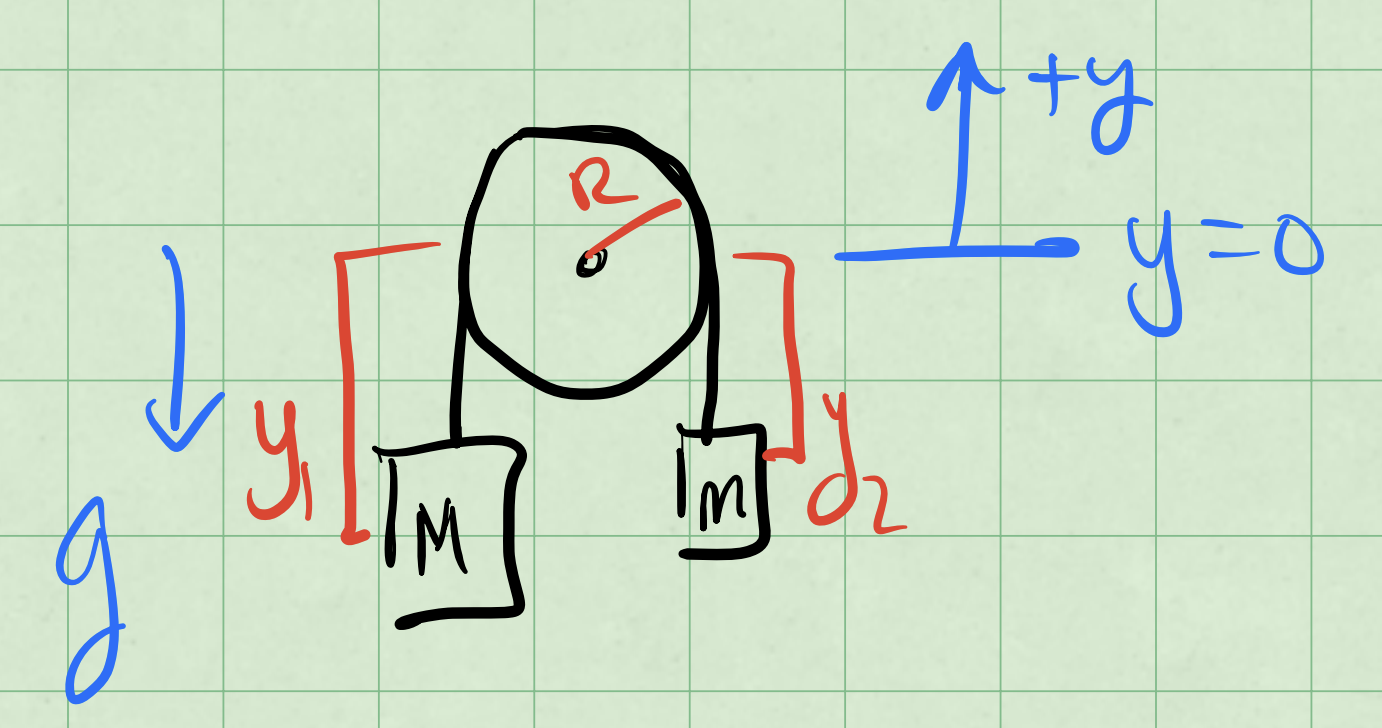
\includegraphics[keepaspectratio,alt={Atwood Machine}]{/Users/caballero/repos/teaching/modern-classical-mechanics/images/notes/week13/atwood.png}}
\caption{Atwood Machine}
\end{figure}

These coordinates are measured from the center of the pulley and
positive \(y_1\) and \(y_2\) are taken to be upward. Let's try to use
the Lagrangian formalism to find the equations of motion for this
system.

\[V = + Mgy_1 + mgy_2\]

\[T = \dfrac{1}{2}M\dot{y}_1^2 + \dfrac{1}{2}m\dot{y}_2^2\]

\subsubsection{Equation of Constraint}\label{equation-of-constraint}

But notice that \(y_1\) and \(y_2\) are no independent coordinates. If
we unravel the string that is over the pulley, we find that (assume
length of string is \(l\)):

\[y_1 + \pi R + y_2 = l\]

where \(R\) is the radius of the pulley. That is shown in the figure
below.

\begin{figure}
\centering
\pandocbounded{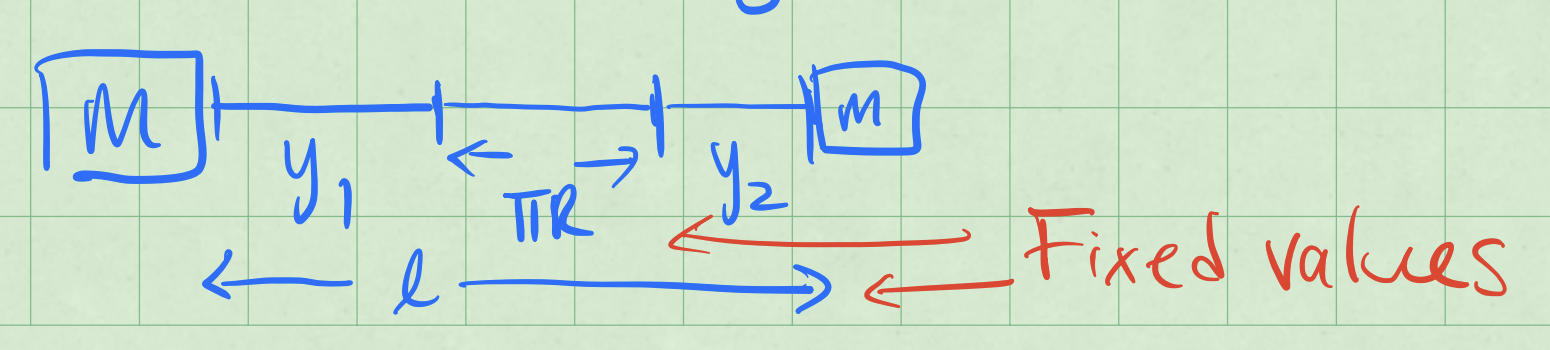
\includegraphics[keepaspectratio,alt={Unraveled String}]{/Users/caballero/repos/teaching/modern-classical-mechanics/images/notes/week13/string-unraveled.png}}
\caption{Unraveled String}
\end{figure}

The equation above is called an \textbf{equation of constraint}. It
relates the coordinates \(y_1\) and \(y_2\) to each other. We can use
this equation to eliminate one of the coordinates. Let's eliminate
\(y_2\):

\[l = y_1 + \pi R + y_2 \rightarrow y_1 = (l - \pi R) - y_2\]

This constraint has implications for velocities,

\[\dfrac{dy_1}{dt} = \dfrac{d}{dt}\left((l-\pi R) - y_2\right) = -\dfrac{dy_2}{dt}\]

\[\dot{y}_1 = -\dot{y}_2.\]

This is likely what we could have expected, that the two masses move in
opposite directions at the same speed.

\subsubsection{Constructing the
Lagrangian}\label{constructing-the-lagrangian}

Let's use this constraint to reduce the number of coordinates in the
Lagrangian.

\[\mathcal{L}(y_1, y_2, \dot{y}_1, \dot{y}_2) \rightarrow \mathcal{L}(y_1, \dot{y}_1)\]

We can do this by substituting \(y_2\) in terms of \(y_1\) into the
energy equations:

\[T(y_1, \dot{y}_1) = \dfrac{1}{2}M\dot{y}_1^2 + \dfrac{1}{2}m\dot{y}_2^2 = \dfrac{1}{2}(M+m)\dot{y}_1^2 = T(\dot{y}_1)\]

\[V(y_1, y_2) = +Mgy_1 + mgy_2\]
\[V(y_1, y_2) = Mgy_1 + mg((l-\pi R) - y_1)\]
\[V(y_1, y_2) = (M-m)g y_1 + mg(l-\pi R)\]
\[V(y_1, y_2) = (M-m)g y_1 + U_0\]

where \(U_0 = mg(l-\pi R)\) is a constant and will not affect the
equations of motion.

\[\mathcal{L}(y_1, \dot{y}_1) = T(\dot{y}_1) - V(y_1) = \dfrac{1}{2}(M+m)\dot{y}_1^2 - (M-m)g y_1\]

\[\dfrac{\partial \mathcal{L}}{\partial y_1} = -(M-m)g\]

\[\dfrac{\partial \mathcal{L}}{\partial \dot{y}_1} = (M+m)\dot{y}_1\]

These derivatives give the following equation of motion:

\[-(M-m) g - \dfrac{d}{dt}\left((M+m)\dot{y}_1\right) = 0\]

\paragraph{Generalized Force}\label{generalized-force}

Notice that the first term in the above equation is the force on the
mass \(M\) in the Newtonian picture: the weight of \(M\) minus the
weight of \(m\). That makes sense because the Lagrangian formalism is
supposed to reproduce Newton's laws, and the spatial derivative of the
Lagrangian produces a
\href{https://en.wikipedia.org/wiki/Generalized_force}{generalized
force}.

\[\dfrac{\partial \mathcal{L}}{\partial q_i} = -\dfrac{\partial V}{\partial q_i} = F_i\]

The kinetic term has no spatial dependence, so it does not contribute to
the generalized force.

\paragraph{Generalized Momentum}\label{generalized-momentum}

The second term in the above equation is the time derivative of the
momentum of the system using \(y_1\) as the coordinate:

\[(M+m)\dot{y}_1 = M\dot{y}_1 - m\dot{y}_2 = p_{y_1}\]

Again, that is a sensible result because the Lagrangian formalism is
supposed to reproduce Newton's laws, and the generalized force is
related to the time derivative of the
\href{https://phys.libretexts.org/Bookshelves/Classical_Mechanics/Variational_Principles_in_Classical_Mechanics_(Cline)/07\%3A_Symmetries_Invariance_and_the_Hamiltonian/7.02\%3A_Generalized_Momentum}{generalized
momentum}.

\[\dfrac{d}{dt}\left(\dfrac{\partial \mathcal{L}}{\partial \dot{q}_i}\right) = \dfrac{d}{dt}\left(\dfrac{\partial T}{\partial \dot{q}_i}\right) = \dfrac{dp_{q_i}}{dt}\]

\subsubsection{Equation of Motion}\label{equation-of-motion}

The equation of motion can be written as

\[(M=m)\ddot{y}_1 = -(M-m)g\] \[\ddot{y}_1 = -\dfrac{(M-m)}{(M+m)}g.\]

With \(M > m\), this acceleration is downward as the larger mass \(M\)
accelerates down. With \(\dot{y}_1 = -\dot{y}_2\), we know
\[\ddot{y}_2 = -\ddot{y}_1\], so that:

\[\ddot{y}_2 = \dfrac{(M-m)}{(M+m)}g\]

Again, with \(M > m\), this acceleration is upward as the smaller mass
\(m\) accelerates up.

\subsection{Example: Atwood Machine with Rotating
Pulley}\label{example-atwood-machine-with-rotating-pulley}

In the previous example, we didn't take into account the energy needed
to rotate the pulley. Let's do that now. Beucase the rope cannot slip,
any small rotation \(Rd\phi\) of the pulley give a change \(dy_1\) in
the position of mass \(M\). This is the
\href{https://en.wikipedia.org/wiki/No-slip_condition}{no slip
constraint}.

If the pulley has a mass \(M_p\) and radius \(R\), then we must
introduce it's kinetic energy:

\[T_{pulley} =  \dfrac{1}{2} I \omega^2\]

where \(I\) is the
\href{https://en.wikipedia.org/wiki/List_of_moments_of_inertia}{moment
of inertia} of the pulley and \(\omega\) is the angular velocity of the
pulley, \(\omega = \dot{\phi}\). This angular velocity is related to the
linear velocities of the masses.

\[I = \dfrac{1}{2}M_p R^2\]

\[T_{pulley} =  \dfrac{1}{2} \left(\dfrac{1}{2}M_p R^2\right) \dot{\phi}^2\]
\[T_{pulley} =  \dfrac{1}{4}M_p R^2 \dot{\phi}^2\]

We now map this additional kinetic energy into the problem.

\[T(\dot{y}_1, \dot{\phi}) = \dfrac{1}{2}(M+m)\dot{y}_1^2 + \dfrac{1}{4}M_p R^2 \dot{\phi}^2\]

But the constraint is such that,

\[\dot{y}_1 = Rd\phi \rightarrow y_1 = R\phi +\underbrace{R\phi_0}_{\textrm{const.}}\]

\[\dot{y}_1 = R\dot{\phi}\]

We work these back into \(T\), \(V\), and \(\mathcal{L}\).

\[T(\dot{\phi}) = \dfrac{1}{2}(M+m)\dot{y}_1^2 + \dfrac{1}{4}M_p R^2 \dot{\phi}^2\]
\[T(\dot{\phi}) = \dfrac{1}{2}(M+m+\frac{1}{2}M_p)R^2 \dot{\phi}^2\]

\[V(\phi) = (M-m)gy_1 + U_0\]
\[V(\phi) = (M-m)g(R\phi + R\phi_0) + U_0\]
\[V(\phi) = (M-m)gR\phi + \tilde{U}_0\]

where \(\tilde{U}_0 = (M-m)gR\phi_0 + U_0\) is another constant that
will not affect the equations of motion.

\[\mathcal{L}(\phi, \dot{\phi}) = T(\dot{\phi}) - V(\phi)\]
\[\mathcal{L}(\phi, \dot{\phi}) = \dfrac{1}{2}(M+m+\frac{1}{2}M_p)R^2 \dot{\phi}^2 - (M-m)gR\phi\]

\subsubsection{Torque and Angular
Momentum}\label{torque-and-angular-momentum}

Our generalized coordinate is \(\phi\) and our generalized velocity is
\(\dot{\phi}\). We apply the Euler-Lagrange equation. We obtain the
generalized force:

\[\dfrac{\partial \mathcal{L}}{\partial \phi} = -(M-m)gR = F_{\phi}\]

Notice that in this case, the generalized force is not the same as the
force on mass \(M\) in the Newtonian picture. It's a torque around the
pulley.

We can find the generalized momentum in a similar way:

\[\dfrac{\partial \mathcal{L}}{\partial \dot{\phi}} = (M+m+\frac{1}{2}M_p)R^2\dot{\phi} = p_{\phi}\]

This is the angular momentum of the system about the axle. We can see
that by breaking down each part and adding them up.

\[\vec{L}_{total} = \vec{L}_{disk} + \vec{L}_{M} + \vec{L}_{m}\]

\[\vec{L}_{disk} = I_{disk}\omega = \dfrac{1}{2}M_p R^2 \dot{\phi}\,\text{(out of the page)}\]

\[\vec{L}_{M} = M\vec{r}_{M}\times \vec{v}_{M} = M(R\hat{r})\times (R\dot{\phi}\hat{\phi}) = MR^2 \dot{\phi}\,\text{(out of the page)}\]

\[\vec{L}_{m} = M\vec{r}_{m}\times \vec{v}_{m} = m(R\hat{r})\times (R\dot{\phi}\hat{\phi}) = mR^2 \dot{\phi}\,\text{(out of the page)}\]

Add them up:

\[\vec{L}_{total} = \left(\dfrac{1}{2}M_p + M + m\right)R^2 \dot{\phi}\,\text{(out of the page)}\]

Or the magnitude:

\[L_{total} = \left(\dfrac{1}{2}M_p + M + m\right)R^2 \dot{\phi}\]
\[p_{\phi} = L_{total}\]

\subsubsection{Equation of Motion}\label{equation-of-motion-1}

We return to the diffeferential equation of motion:

\[-(M-m)gR - \dfrac{d}{dt}((M+m+\frac{1}{2}M_p)R^2\dot{\phi} = 0\]
\[-(M-m)gR - (M+m+\frac{1}{2}M_p)R^2\ddot{\phi} = 0\]

which produces the following equation of motion:

\[\ddot{\phi} = -\dfrac{g}{R}\dfrac{(M-m)}{(M+m+\frac{1}{2}M_p)}\]

which is a constant acceleration.

    \subsection{Example: Bead in a Parabolic
Bowl}\label{example-bead-in-a-parabolic-bowl}

A bead of mass \(m\) is constrained to move along a parabolic bowl.
There is a gravitational force acting on the bead. The bowl is symmetric
about the \(z\)-axis and the bead is constrained to move along the
surface without friction or rolling. The bowl is described by the
equation:

\[z = \dfrac{1}{2}c(x^2 + y^2)\]

where \(c\) is a constant that describes the curvature of the bowl. The
figure below shows the system.

\begin{figure}
\centering
\pandocbounded{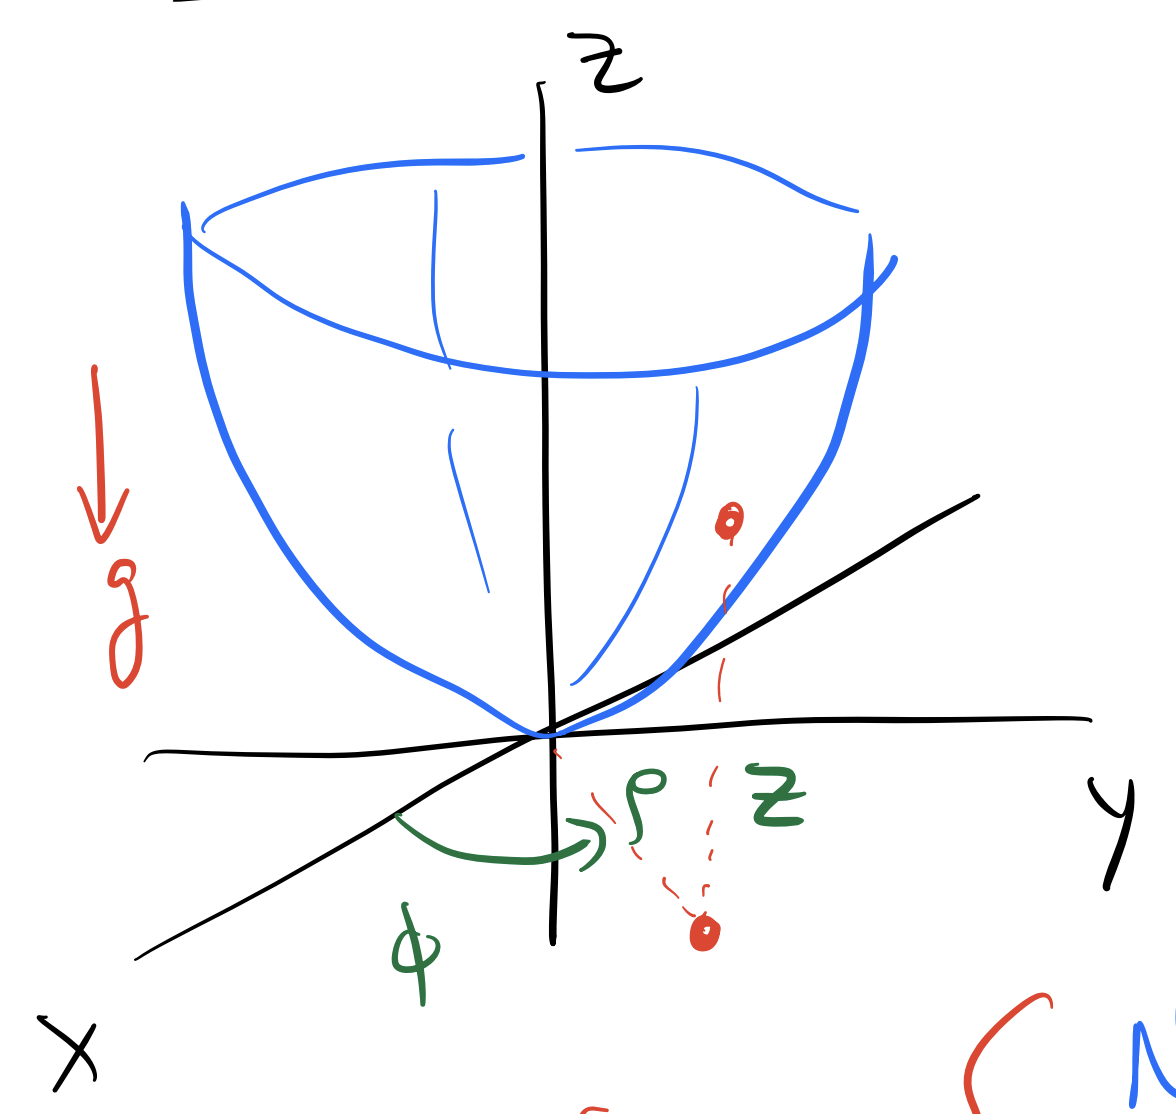
\includegraphics[keepaspectratio,alt={Bead in a Parabolic Bowl}]{/Users/caballero/repos/teaching/modern-classical-mechanics/images/notes/week13/paraboloid.png}}
\caption{Bead in a Parabolic Bowl}
\end{figure}

In this case the system is better solved in cylindrical coordinates. The
coordinates are \((r, \phi, z)\), where \(r\) is the distance from the
\(z\)-axis, \(\phi\) is the angle around the \(z\)-axis, and \(z\) is
the height above the \(xy\)-plane as shown above.

With \(\langle \rho, \phi, z\rangle\) as the coordinates, equation for
the constraint is:

\[z = \dfrac{1}{2}c(x^2 + y^2) = \dfrac{1}{2}c\rho^2.\]

Note that \(c\) has units.

\[[z] = m \quad [\rho^2] = m^2 \quad [c] = \dfrac{1}{m}\]

The speed in cylindrical coordinates can be derived from the expressions
in Cartesian coordinates, but we quote the result here:

\[v^2 = \dot{\rho}^2 + \rho^2\dot{\phi}^2 + \dot{z}^2.\]

\subsubsection{Constructing the
Lagrangian}\label{constructing-the-lagrangian}

We write the kinetic and potential energy of the bead in terms of the
coordinates \((r, \phi, z)\).

\[T = \dfrac{1}{2}m\left(\dot{\rho}^2 + \rho^2\dot{\phi}^2 + \dot{z}^2\right)\]

\[V = mgz\]

In principle, the Lagrangian can depend on all three coordinates and all
three velocities.

\[\mathcal{L}(\rho, \dot{\rho}, \phi, \dot{\phi}, z, \dot{z}, t) = T - V\]

There is no explicit time dependence, so we can ignore \(t\). When the
Lagrangian has no explicit time dependence, we should expect the energy
to be conserved. This form of Lagrangian analysis does not account for
dissipation.

\[\mathcal{L}(\rho, \dot{\rho}, \phi, \dot{\phi}, z, \dot{z})\]

Moreover, with the symmetry of the problem, we can expect no \(\phi\)
dependence. That is the gravitational potential energy only depends on
\(z\) and not on \(\phi\). This is a consequence of the symmetry of the
problem and indicates that \(\phi\) is a
\href{https://phys.libretexts.org/Bookshelves/Classical_Mechanics/Variational_Principles_in_Classical_Mechanics_(Cline)/07\%3A_Symmetries_Invariance_and_the_Hamiltonian/7.05\%3A_Cyclic_Coordinates}{cyclic
coordinate}. We thus expect angular momentum to be conserved about the
\(z\)-axis.

\[\mathcal{L}(\rho, \dot{\rho}, \dot{\phi}, z, \dot{z})\]

Lastly, the constraint equation gives us \(z\) in terms of \(\rho\):

\[z = \dfrac{1}{2}c\rho^2\]

And thus we can find the time derivative of \(z\):

\[\dot{z} = 2c\rho\dot{\rho}.\]

So the Lagrangian can be simplified three variables:

\[\mathcal{L}(\rho, \dot{\rho}, \dot{\phi}) = T - V\]

\[\mathcal{L}(\rho, \dot{\rho}, \dot{\phi}) = \dfrac{1}{2}m\left(\dot{\rho}^2 + \rho^2\dot{\phi}^2 + 4c^2\rho^2\dot{\rho}^2\right) - mg\dfrac{1}{2}c\rho^2\]

\subsubsection{Equations of Motion}\label{equations-of-motion}

We can now apply the Euler-Lagrange equations to find the equations of
motion. We will do this for each coordinate. Let's start with \(\phi\)
because there is only one term in the Lagrangian that depends on
\(\dot{\phi}\).

\[\underbrace{\dfrac{\partial \mathcal{L}}{\partial \phi}}_0 - \dfrac{d}{dt}\left(\dfrac{\partial \mathcal{L}}{\partial \dot{\phi}}\right) = 0\]

\[\dfrac{d}{dt}\left(\dfrac{\partial \mathcal{L}}{\partial \dot{\phi}}\right) = \dfrac{d}{dt}\underbrace{\left(m\rho^2\dot{\phi}\right)}_{L_z} = 0\]

This equation of motion indicates that the angular momentum about the
\(z\)-axis is conserved, as we expected from the symmetry of the
problem.

For the coordinate \(\rho\), we have:

\[\dfrac{\partial \mathcal{L}}{\partial \rho} - \dfrac{d}{dt}\left(\dfrac{\partial \mathcal{L}}{\partial \dot{\rho}}\right) = 0\]

\[\dfrac{\partial \mathcal{L}}{\partial \rho} = m\rho\dot{\phi}^2 + 4c^2m\rho\dot{\rho}^2 - 2mgc\rho\]

\[\dfrac{\partial \mathcal{L}}{\partial \dot{\rho}} = m\dot{\rho} + 4mc^2\rho^2\dot{\rho}\]

\[\dfrac{d}{dt}\left(\dfrac{\partial \mathcal{L}}{\partial \dot{\rho}}\right) = m\ddot{\rho} + 8mc^2\rho\dot{\rho}^2 + 4mc^2\rho^2\ddot{\rho}\]

We can now write the equation of motion:

\[m\rho\dot{\phi}^2 + 4c^2m\rho\dot{\rho}^2 - 2mgc\rho - m\ddot{\rho} - 8mc^2\rho\dot{\rho}^2 - 4mc^2\rho^2\ddot{\rho} = 0\]

We can clean this up a little bit:

\[\ddot{\rho}(1+4c^2\rho^2) + 8c^2\rho\dot{\rho}^2 = \rho\dot{\phi}^2 + 4c^2\rho\dot{\rho}^2 - 2gc\rho\]

\[\ddot{\rho}(1+4c^2\rho^2) + 4c^2\rho\dot{\rho}^2 - \rho\dot{\phi}^2 + 2gc\rho = 0\]

We try to write both equations in terms of their accelerations. We have:

\[\ddot{\rho} = -\dfrac{4c^2\rho\dot{\rho}^2 - \rho\dot{\phi}^2 + 2gc\rho}{1+4c^2\rho^2}\]

\[\ddot{\phi} = - \dfrac{2\rho\dot{\rho}\dot{\phi}}{\rho^2}\]

For which we can develop a solution anywhere away from the origin
(\(\rho \neq 0\)).

\subsubsection{Preparing for Numerical
Solution}\label{preparing-for-numerical-solution}

We need to write these equations in a form that is ready for numerical
solution. We can do this by writing the equations in terms of the first
derivatives. Let \(\omega = \dot{\phi}\) and \(v = \dot{\rho}\). We get
4 1st order equations:

\[\dot{\rho} = v\] \[\dot{\phi} = \omega\]
\[\dot{v} = -\dfrac{4c^2\rho v^2 - \rho\omega^2 + 2gc\rho}{1+4c^2\rho^2}\]
\[\dot{\omega} = - \dfrac{2 v\omega}{\rho^2}\]

    


    % Add a bibliography block to the postdoc
    
    
    
\end{document}
